


\section{Soundness of our proof system}

\subsection{Definitions}

We will define the {\emph {meaning}} of  $M\ \vdash\  \{\, A \,  \}\ e\  \{\, A' \, \}$ triples in the usual way, \ie that execution of $e$ least to a state which satisfies $A'$. For this definition we also need the new execution relation\footnote{TODO: This is what we used to call $\leadstoUp$, the definition slightly different} ...
Namely, \ $\leadstoRec {M} {\sigma_1} {\sigma} {\sigma_2}$\  expresses that $\sigma_1$ leads to $\sigma_2$ provided
 that the top frame from $\sigma$ is never popped. This relation talks about executions where we push and pop frames on top of the stack in $\sigma$, but never pop the top frame in $\sigma$'s stack. Moreover, $\leadstoFin {M} {\sigma} {\sigma'}$  expresses that the frame on top of $\sigma$ executes to completion and reaches $\sigma'$.
We require that $\sigma'.cont$ is a value in order to ensure that the continuation in $\sigma$ has terminated. \footnote{ \sd{TODO: Also, will need add more requirements  -- or use different rewrite relation --- to ensure that we did not pop the top frame}.}
 
{
\begin{definition}[Terminating semantics]
\label{def:term}
We define the relation  ...
\begin{itemize}
\item
$\Final {\sigma}$ \ \ \ iff \ \ \  $\exists \phi. [\ \sigma = (\phi\cdot\_,\_) \ \wedge \ \phi.\texttt{cont} \in \Values \ ]$
\item
$\leadstoFin {M} {\sigma} {\sigma'}$ \ \ \ P \ \ \  $\leadstoRecStar {M} {\sigma} {\sigma} {\sigma'} \ \wedge \ \ \Final{\sigma'}$.
\end{itemize}
\end{definition}
}

We define the semantics of Hoare triples in the usual way (note that we do not use the observable states semantics here): 

\begin{definition}[Semantics of Hoare triples]

 
For modules $M$, and assertions $A$, $A'$   we define the semantics of Hoare-triples, 
 $M\ \models\  \{\, A \,  \}\ e\  \{\, A' \, \}$ as follows:
\begin{itemize}
\item
$M\ \models\  \{\, A \,  \}\ e\  \{\, A' \, \}$ \\
iff\\
 for a all $M'$, for all $\sigma$ such that \sd{$\arising \sigma {M\circ M'}$}\footnote{TAKE NOTE here} \\
$\strut ~ ~ ~ ~ [ \ \ M,\sigma \ \models \ A \ \wedge\  
 \sigma.cont$=$e$ $\ \ \wedge\  \ \leadstoFin  {M\circ M'} \sigma {\sigma'}$
 \\
$\strut ~ ~ ~ ~ \ \  \ \ \Longrightarrow$ \\
$\strut ~ ~ ~ ~ \ \ M,\sigma' \ \models \ A'\ \ ]$
\end{itemize}
\end{definition}
 

Below, we define soundness of a Hoare logic in the classical way:

\begin{definition}[Soundness of Hoare logic]

 
Assume a judgement $\vdash \ \subseteq Module \times Assertion \times Expression \times Assertion$ of the form
$\_ \ \vdash\  \{\, \_ \,  \}\ \_ \  \{\, \_ \, \}$.\\
\begin{itemize}
\item
The judgement $\_ \ \vdash\  \{\, \_ \,  \}\ \_ \  \{\, \_ \, \}$ is {\emph {sound}}, \\ iff \\
for all modules $M$, expression $e$, and assertions $A$, $A'$:\\
$\strut\hspace{3cm} \ M\ \vdash\  \{\, A \,  \}\ e\  \{\, A' \, \}$ \ \ \  implies\ \ \ 
 $M\ \models\  \{\, A \,  \}\ e\  \{\, A' \, \}$.
\end{itemize}
 \end{definition}
 
 
 \subsection{Preliminaries for Proving Soundness of our Hoare Logic}
 
 \subsubsection{Requirements}
 
 
 \begin{definition}[Inversion] We say that our Hoare logic has the \emph{ inversion} property if it satisfies the  following:
 \begin{enumerate}
 \item
 $ M\ \vdash\  \{\, A \,  \}\ e_1; e_2 \  \{\, A' \, \}$\\
 $\strut \hspace{2cm}\ \Longrightarrow M\ \vdash\  \{\, A \,  \}\ e_1  \  \{\, A'' \, \}$ \ and \ $M\ \vdash\  \{\, A'' \,  \}\ e_1  \  \{\, A' \, \}$ \ for some $A''$.
 \item
 $ M\ \vdash\  \{\, A \,  \}\ \texttt{if}\ A''\ \texttt{then}\ e_1\ \texttt{else}\ e_2 \  \{\, A' \, \}$\\
 $\strut \hspace{2cm}\ \Longrightarrow
  \ \ \ \ M\ \vdash\  \{\, A\wedge A'' \,  \}\ e_1  \  \{\, A' \, \}$ \ and \ $M\ \vdash\  \{\, A\wedge \neg(A'') \,  \}\ e_2  \  \{\, A' \, \}$  
   \item
$ M\ \vdash\  \{\, A \,  \}\ \texttt{while}\ A''\ \texttt{do}\ e\  \{\, A' \, \}$\\
 $\strut \hspace{2cm}\ \Longrightarrow
  \ \ \ \ ... $  
   \item
...

 \end{enumerate}
 \end{definition}
 
 
 \subsubsection{More Properties}
 
% We need a new execution relation xxxx where $\leadstoLoc {M}  {\sigma_1} {\sigma} {\sigma_2}$ describes execution in the same frame. Namely, the stacks of $\sigma_1$, $\sigma_2$ and $\sigma$ may only differ in the contents of the top frame. Moreover, if $\sigma_1$'s continuation was a method call, then $\sigma_2$ will be the result of that method call. In some sense, we apply  large steps for method calls, and small steps for all other steps.

%\begin{definition}
%We define the relation $\leadstoLoc {M}  {\sigma_1} {\sigma} {\sigma_2}$ which ...
%\begin{itemize}
%\item
%$\leadstoLoc {M} {\sigma_1} {\sigma} {\sigma_2}$ \ \ \ iff \ \ \  $ \exists \phi,\phi_1, \phi2,\psi, $\\
%$\strut  \hspace{2.7cm} [ \ \sigma = (\phi\cdot\psi, \_)\ \wedge \ 
%\sigma_1 = (\phi_1\cdot\psi, \_)  \ \wedge  \ \sigma_2 = (\phi_2\cdot\psi, \_) $\\
%$\strut  \hspace{3.3cm} \wedge $\\
%$\strut  \hspace{2.7cm} \ \ \  [ \ \ \sigma_{1}  \leadsto \sigma_2 \   $ \\
%$\strut  \hspace{3.4cm} \vee$\\
%$\strut \hspace{2.7cm} \ \ \ \ \ \ \exists \phi_{c}, \sigma_{3}, \sigma_{4} [\   \sigma_{3} =  (\phi_{c}\cdot\phi\cdot\psi, \_) \ \wedge \
%M,  \sigma_1 \leadsto \sigma_{3}  \leadsto^*_{! \sigma_{3}}   {\sigma_{4}}   \leadsto \sigma_2\ ]  \ \ ]$
%\end{itemize}
%\end{definition}
%
%Note that $\leadstoLoc M {\sigma_1} {\sigma} {\sigma_2}$  does not imply $\leadstoRec M {\sigma_1} {\sigma} {\sigma_2}$, nor the other way round.

We require that execution is cycle-free:
 \begin{definition}[Cycle-free]
Our underlying language is cycle-free iff for all $M$ and states $\sigma$, $\sigma'$, we have
\begin{itemize}
\item
$ M, \sigma \leadsto^+ \sigma' $ \ \ \ implies \ \ \  $\neg\ (M, \sigma' \leadsto^* \sigma )$
\end{itemize}
\end{definition}

And the following lemma expresses that ..

\begin{lemma}
\label{lemma:subexp}
For any module $M$, expressions $e_1$, $e_2$, and state $\sigma$ and $\sigma'$
\\
if \\
$\strut \ \ \ \ \ \leadstoFin {M} {\sigma} {\sigma'} \ \ \wedge \sigma.\texttt{cont} = e_1; e_2$
\\
then, there exists a $\sigma'''$ such that\\
%
$\strut \ \ \ \ \ \leadstoFin {M} {\sigma[\texttt{cont}\mapsto e1]} {\sigma} {\sigma'''} \ \ \wedge \ \ %\leadstoFin {M} {\sigma''} {\sigma'} \ \wedge \ \  \sigma''.\texttt{cont} = e_2 \ \ \wedge$\\
%$\strut \ \ \ \ \ \leadstoFin {M} {\sigma[\texttt{cont}\mapsto e1]}   {\sigma'''}  \ \ \wedge \ \ 
\leadstoFin {M} {\sigma'''[\texttt{cont}\mapsto e2]}   {\sigma'} $
% \sigma''$ isomorphic to $\sigma'''$ up to the continuation of top frame
\end{lemma}
 

 The following lemma says that a terminating execution $\leadstoFin {M} {\sigma} {\sigma'}$ of an external call in $\sigma$ consists of a sequence of (sequences of external states inteleaved with terminating executions in internal states:
 
\begin{lemma}
\label{lemma:external_breakdown}[Summarised Execution]
For any module $M$,  states $\sigma$ and $\sigma'$:
\\
if \\
$\strut \ \ \ \ \ \leadstoFin {M} {\sigma} {\sigma'}  \ \ \wedge\ \ \sigma.\texttt{cont} = y.m(\overline y) \ \ \wedge  \ \ M,\sigma \models \internal {\texttt{this}}\ \ \wedge \ \ M,\sigma \models \external y\ $
\\
then
\\
$\strut \ \ \ \ \ \exists n,m\in \mathbb{N}, \sigma_1, ... \sigma_n \in States, i_1,...i_m \in \mathbb{N}. [$\\
$\strut \ \ \ \ \ \ \ \ \ \ \sigma=\sigma_1  \ \wedge  \sigma_n=\sigma'\ \wedge\ \  i_1=2 \ \ \wedge\ \   i_m=n\ \ \wedge$\\
$\strut \ \ \ \ \ \ \ \ \ \ \ \forall j\in [1..m].$\\
$\strut \ \ \ \ \ \ \ \ \ \ \hspace{.8cm}[ \ i_j \in [1..n]\  \wedge \ i_{j}+3  < i_{j+1} \ \ \wedge$\\
$\strut \ \ \ \ \ \ \ \ \ \ \hspace{1cm} M, \sigma_{i_j+1} \models \internal {\texttt{this}}  \ \ \wedge \ \ M, \sigma_{i_j+2} \models \internal {\texttt{this}}  \ \ \wedge$\\
$\strut \ \ \ \ \ \ \ \ \ \ \hspace{1cm}  \leadstoFin {M} {\sigma_{i_j+1}} {\sigma_{i_j+2}}\ \ \wedge $\\
$\strut \ \ \ \ \ \ \ \ \ \ \hspace{1cm} \forall k\in [i_j+3..i_{j+1}]. [\ M, \sigma_k \models \external {\texttt{this}}  \ \ \wedge \ \ \leadstoRec {M}  {\sigma_{k}} {\sigma}{\sigma_{k+1}}] \ \ ]$
\end{lemma}

The meaning of lemma \ref{lemma:summaries} is illustrated through an example in Fig. \ref{fig:summaries}.

\begin{figure}[htb]
\begin{tabular}{c}
\hline \\
the original execution:
\\
~ \\
\resizebox{9cm}{!}
{
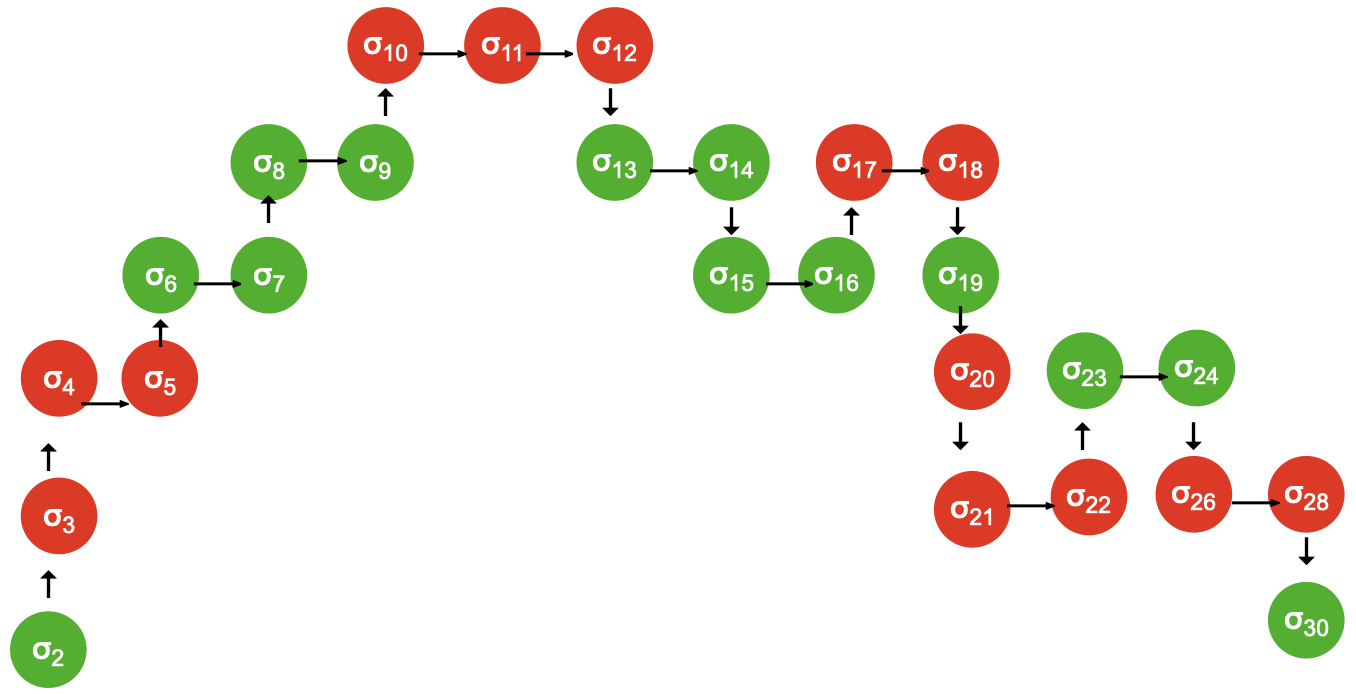
\includegraphics[width=\linewidth]{diagrams/summaryA.png}
} 
\\
\hline \\
the summarised execution:
\\
~ \\
\resizebox{9cm}{!}
{
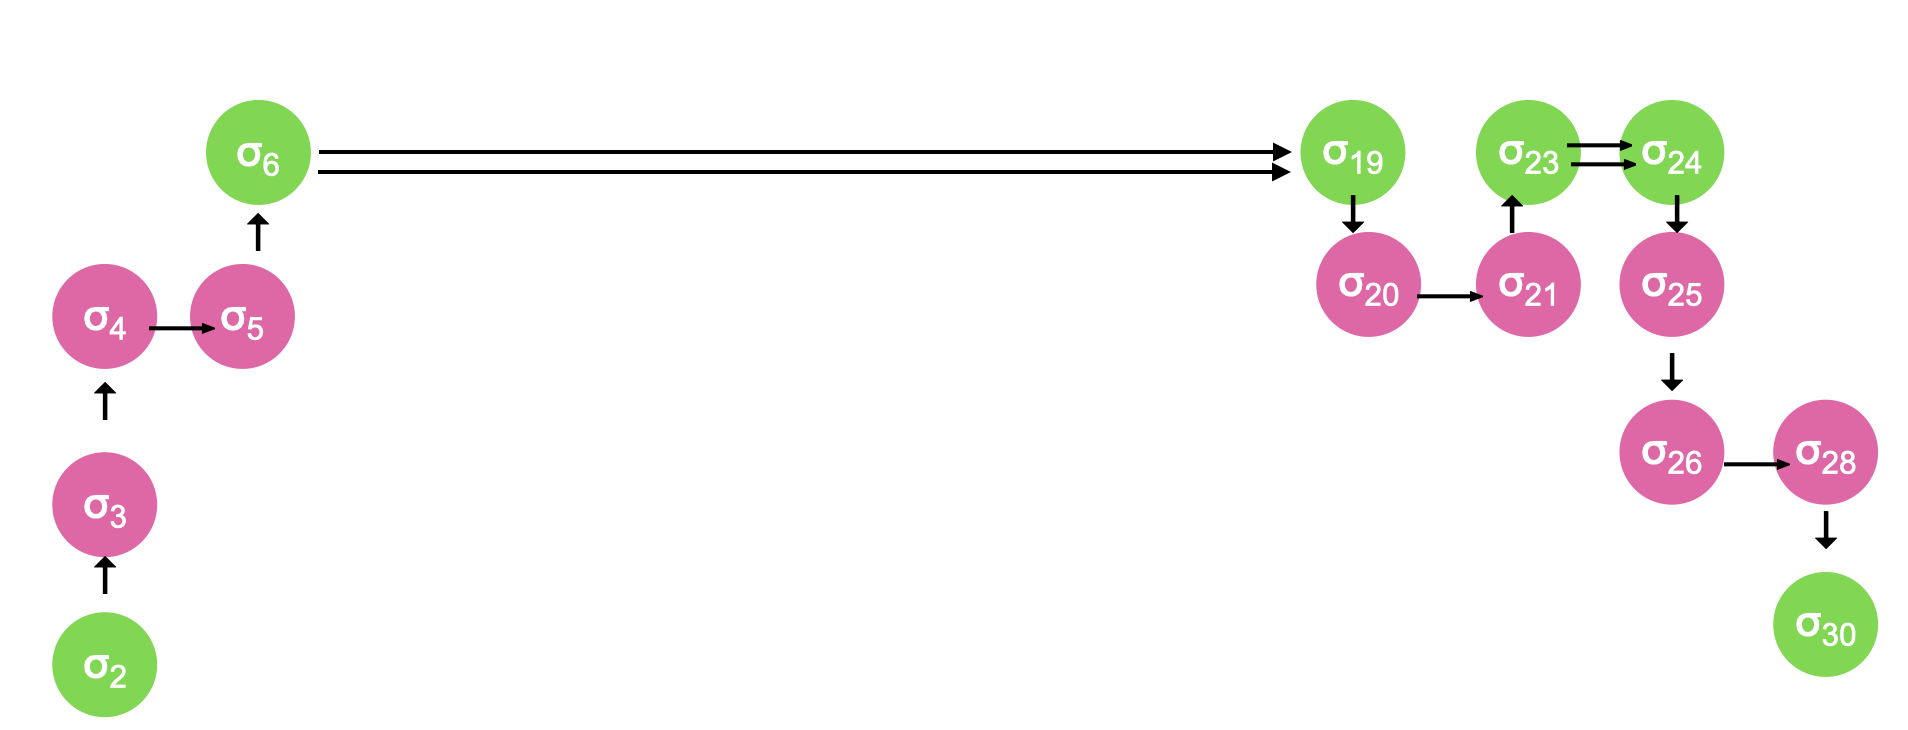
\includegraphics[width=\linewidth]{diagrams/summaryB.png}
} 
\\
\hline \hline
\end{tabular}
   \caption{Summaries. 
   }
   \label{fig:summaries}
 \end{figure}

We now define a well-founded ordering on states, which we will use in the proof of soundness of our Hoare logic. 

\begin{definition}
For module $M$ and states $\sigma$, $\sigma'$, we define
\begin{itemize}
\item $\sigma' \ll_M  \sigma$ \ \ \ iff \ \ \ $\leadstoRecStar {M} {\sigma} {\sigma} {\sigma'}$ and $\sigma\neq \sigma'$\\
$\strut \hspace{2cm} \ \ $ or $\\
$\strut \hspace{2cm} \ \ $\sigma.\texttt{cont}=e_1; e_2 \ \ \ \wedge \ \ \ \ \sigma'=\sigma.[\texttt{cont}\mapsto e_1]$
\end{itemize}
\end{definition}

\begin{lemma}
If our language has the acyclic property, then $\ll_M$ is a well-founded ordering.
\end{lemma}

TODO: revisit the lemma above. Need to show that there are no infinite descending chains.

\subsection{Proving Soundness of the Hoare Logic}

We take two modules $M$ and $M'$ arbitrary. We define the following property of states:

$Q(\sigma)\ \ \ \triangleq\  \ \ \forall A, A'. $\\
$\strut \hspace{2cm} [ \  \ Arising(\sigma,M*M') \ \  \wedge\ \ 
% $\\$\strut \hspace{2cm}  \ \ \  \ 
M \vdash \{A \} \sigma.\texttt{cont} \{A' \} \ \ \wedge\ \  M, \sigma \models  A \ \ 
\wedge\ \  \leadstoFin  {M*M'}{\sigma}  {\sigma'}$\\
$\strut \hspace{2cm}   \ \  \Longrightarrow$\\
$\strut \hspace{2cm} \ \   \ \ M, \sigma' \models  A'  \  \ ]$

\noindent
We assume that: \\
$\strut \ \ \ (*) \ \ M \models HS(M)$
where $HS$ also includes Hoare triples for methods.\\
We will prove that \\
$\strut \ \ \ (**) \ \ \forall \sigma.[  \ \ Q(\sigma)\ \ ]$
\\
The proof is by induction on $\sigma$ using the ordering $\ll_{M*M'}$. 

\noindent
\vspace{.2cm}
  {\textbf{Proof Sketch}} 
We start by case analysis on $\sigma.\texttt{cont}$ 

\begin{description} 
\item[$e\ \equiv\ x=y $] 

By standard Hoare logic arguments (or even parametric) ...
\item[$e\ \equiv\ x=y.f $] 

By standard Hoare logic arguments (or even parametric) ...

 \item[$e\ \equiv\ y.m(\overline y)$]  
and $y$ is internal. 

We construct the new frame for the call, $\sigma''$. We obtain that $\sigma'' \ll_{M*M'} \sigma$. We also have that  $ \leadstoFin  {M*M'}{\sigma''}  {\sigma'}$, and $\sigma''$ "returns to $\sigma'$.
We apply the IH to $\sigma''$ and knowledge from Hoare loci rules, and are done.  

\item[$e\ \equiv\ y.m(\overline y)$]  and $y$ is external. 
\\
We apply the rule for external calls, and obtain that the argument hinges on a requirement that there is an invariant property $A''$, which is lifted to the first external call, and will we need to demonstrate is preserved by al enclosed call internal or external, and this $A''$ must be valid at the last external frame, and is then lowered to the current frame.
\\
We apply lemma \ref{lemma:external_breakdown}. In terms of the example in Fig. \ref{fig:summaries} we are now working with the summarised execution, \ie the execution of the methods in $\sigma_8$ and 
$\sigma_{22}$ is summarised into one large step.
Regardless of example, obtain that the first external calls ($\sigma_2$, ... $\sigma_{j_2}$) all preserve $A''$ because it is encapsulated. 
Therefore $A''$ also holds at $\sigma_{j_2}+1$. 
Since we have (*), we know that $A''$ has been proven as an invariant of all external methods, and therefore, by applying the (H), we obtain that $A''$ holds at $\sigma_{j_2} + 3$  (In terms of our example in Fig. \ref{fig:summaries}  $A''$ would hold in $\sigma_{24}).$ 
We continue in the same vain, until we reach $\sigma_{n-1}$ (that is $\sigma_{28}$ in our example), and then we apply the Hoare rule and what we know about lowering.
 \item[$e\ \equiv e_1; e_2$ ]
 By lemma \ref{lemma:subexp} we can break execution to two parts. For the second part we can apply the IH. But for the first part is looks as if we are repeating the work from earlier cases. OR... should we extend the def of $\\ll_M$ so that $\sigma[\texttt{cont}\mapsto e_1] \ll_M \sigma$.
\end{description}


\vspace{1cm}

Finally, we can now prove soundness of the overall system

\begin{theorem}[Soundness]
\label{thm:soundness}
Assume a a sound \SpecO proof system, $\proves{M}{A}$, 
a sound encapsulation inference system, $\proves{M}{\encaps{A}}$,
 and  that on top of these systems we built
 the \SpecLang logic according to the rules in Figures \ref{f:classical->singlestep},  \ref{f:only-if-single}, 
 \ref{f:only-through},  and \ref{f:only-if},   then, for    all modules $M$, and all \SpecLang specifications  $S$:
 
 $$\proves{M}{S}\ \ \ \ \ \ \ \mbox{implies}\ \ \ \ \ \  \ \ \ \satisfies{M}{S}$$
\end{theorem}

\begin{proof}
follows from earlier theorem
% by induction on the derivation of $\proves{M}{S}$.
\end{proof}
 


Theorem. \ref{thm:soundness} demonstrates 
 that the   \SpecLang logic is sound with respect to the semantics of \SpecLang specifications.
 The \SpecLang logic parametric wrt to the algorithms for proving validity of assertions
 $\proves{M}{A}$, and 
 assertion encapsulation ($\proves{M}{\encaps{A}}$), and is sound
 provided that these two proof systems are sound.

